% !Mode:: "TeX:UTF-8"

\documentclass[a4paper,11pt,onecolumn,twoside]{article}
\usepackage{fancyhdr}
\usepackage{amsmath,amsfonts,amssymb,amsthm}
\usepackage{graphicx}
\usepackage{verbatim}
\usepackage{mathptmx}
\usepackage{booktabs}
\usepackage[labelfont=bf]{caption}
\usepackage{indentfirst}
\usepackage{caption}
\usepackage{setspace}
\usepackage{enumitem}
\usepackage{subfigure}
\usepackage{fontspec}
\usepackage{appendix}
\usepackage{listings}
\usepackage{xcolor}
\lstset{
    numbers=left, 
    numberstyle= \tiny, 
    keywordstyle= \color{ blue!70},
    commentstyle= \color{red!50!green!50!blue!50}, 
    frame=shadowbox, % 阴影效果
    rulesepcolor= \color{ red!20!green!20!blue!20} ,
    escapeinside=``, % 英文分号中可写入中文
    xleftmargin=2em,xrightmargin=2em, aboveskip=1em,
    framexleftmargin=2em
} 
\usepackage{xeCJK}
\newtheorem{lemma}{引理}[section]% Please change the following fonts if they are not available.
\setmainfont{Times New Roman}
 \renewcommand{\contentsname}{目录}
 \renewcommand{\listfigurename}{插图目录}
 \renewcommand{\listtablename}{表格目录}
 \renewcommand{\refname}{参考文献}
 \renewcommand{\abstractname}{摘要}
 \renewcommand{\indexname}{索引}
 \renewcommand{\tablename}{表}
 \renewcommand{\figurename}{图}

\addtolength{\topmargin}{-54pt}
\setlength{\oddsidemargin}{-0.9cm}
\setlength{\evensidemargin}{\oddsidemargin}
\setlength{\textwidth}{17.00cm}
\setlength{\textheight}{24.50cm}

\renewcommand{\baselinestretch}{1.1}
\parindent 22pt

\title{\textbf{GNU SL库帮助文档}}
\author{
马宇恒
\\[2pt]
{\small \textit{匡亚明学院 171240510}}}
\date{}
\fancypagestyle{firststyle}
{
   \fancyhf{}
   \fancyhead[C]{GSL帮助文档}
   \fancyhead[R]{\thepage}
}


\pagestyle{fancy}
\fancyhf{}

\fancyhead[LE,RO]{\thepage}
\fancyhead[CE]{数值计算实验}
\fancyhead[RE]{GSL帮助文档}
\fancyhead[CO]{数值计算实验}
\fancyhead[LO]{GSL帮助文档}

\setlist{nolistsep}
\captionsetup{font=small}

\newcommand{\supercite}[1]{\textsuperscript{\cite{#1}}}
\begin{document}
\maketitle

\tableofcontents
\newpage
\thispagestyle{firststyle}
\setlength{\oddsidemargin}{ 1cm}
\setlength{\evensidemargin}{\oddsidemargin}
\setlength{\textwidth}{15.50cm}
\vspace{-.8cm}


\setcounter{page}{1}

\setlength{\oddsidemargin}{-.5cm}  % 3.17cm - 1 inch
\setlength{\evensidemargin}{\oddsidemargin}
\setlength{\textwidth}{17.00cm}

GNU SL是一个免费的C语言数值计算例程集合。数值计算课程中曾经需要直接调用一部分功能,包含且不限于
\begin{itemize}
\item 常用数学函数与常数
\item 复数
\item 多项式
\item 特殊函数
\item 向量、矩阵和线性代数
\item $\cdots$
\end{itemize}
\par
此外,一些功能是课程本身的实现目标,可以使用GSL库进行验证性工作,包含且不限于
\begin{itemize}
\item 数值积分
\item 差值
\item 一般方程数值解
\item 线性方程组
\item $\cdots$
\end{itemize}
\par
本文将会介绍这些可能用到的功能。虽然这些功能可以使用Matlab等高级语言轻松实现,但作为C/C++的一个功能强大的数学库,学习GSL仍然具有一定意义。在某些领域,C/C++具有的速度和安全性优势使得GSL仍然有着相当多的使用。我第一次接触GSL也是因为处理的问题使用Matlab运算速度低的可怕。GSL的相关声明以及反馈途径见官方网站$$http://www.gnu.org/software/gsl/gsl.html  .$$

本文接下来的命令行操作将以\$作为标志。
\section{下载与安装}
\subsection{下载}
在 http://mirrors.ibiblio.org/gnu/ftp/gnu/gsl/或者其他镜像下载最新的GSL包及其认证文件。下载完成后跟随install.txt里的指示完成安装,步骤如下:
\begin{itemize}
\item 打开命令行。(接下来的每步操作之后需要等待运行完成)
\item 输入$\$ \; cd \; \,location$。location为源代码的文件夹路径(例:/Users/mayuheng/Desktop/gsl)
\item 输入$\$ \; ./configure$
\item 输入$\$\;make$
\item 输入$\$\;make\;check$。若测试结果均为pass且命令行正常运行,可以继续。(耗时可能较长,一般可以跳过)
\item 输入 $\$\; make\;install$
\item 安装完成
\end{itemize}
\par
不过该安装过程默认将库安装在/usr/local/bin 目录下面,如果要成功调用还需要进行操作。
本文以MACOS10.14,XCODE9.3为例说明,其他平台和编译器请自行查询对应操作。
\subsection{调用头文件}
最便捷的操作方式是如图1添加include读取路径。
\begin{enumerate}
\item 选择你的项目
\item 找到Build Setting.
\item 找到Search Paths.
\item 找到Header Search Paths.
\item 单机右侧输入你所安装GSL的路径,一般默认是/usr/local/include,可以在README中查看。
\end{enumerate}
\begin{figure}[htbp]
  \centering
  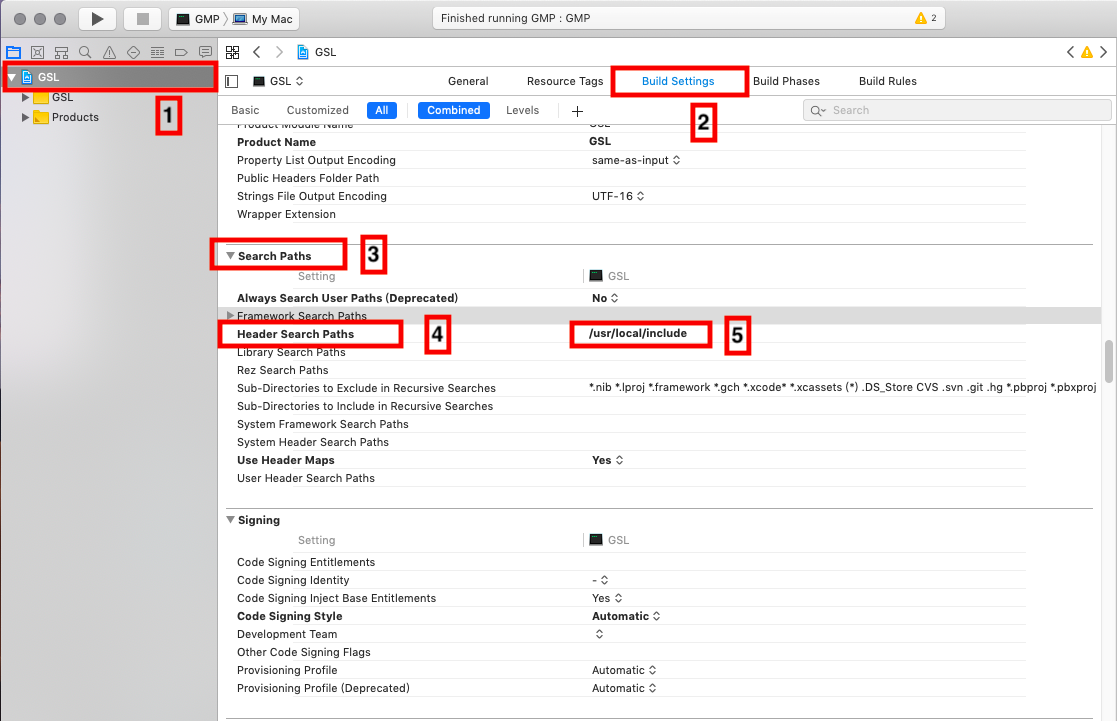
\includegraphics[width=0.8\textwidth]{figures/1.png}
  \caption{调用头文件示意} \label{pngsample}
\end{figure}
\subsection{连接库}
\begin{figure}[htbp]
  \centering
  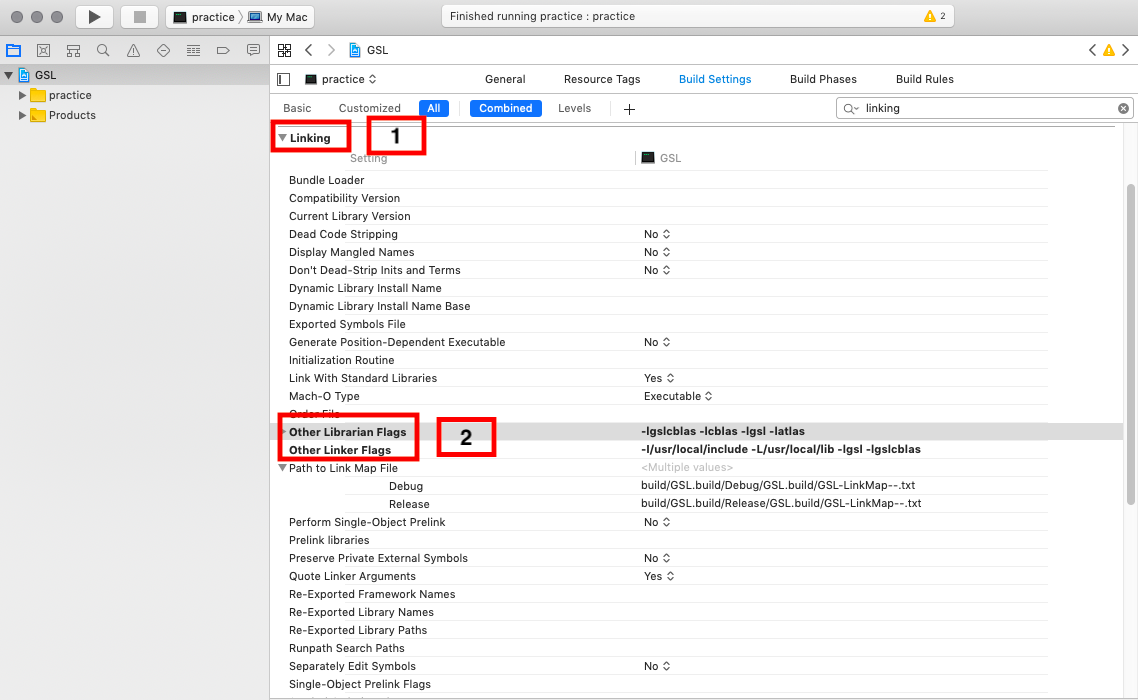
\includegraphics[width=0.75\textwidth]{figures/2.png}
  \caption{连接库示意} \label{pngsample}
\end{figure}
\begin{enumerate}
\item 在同一菜单下找到Linking
\item 找到Other Librarian Flags 和 Other Linker Flags
\item 单击右侧,在Other Librarian Flags 中添加-lgslcblas、-lcblas、-lgsl、-latlas
\item 单击右侧,在Other Linker Flags中添加-I/usr/local/include、-L/usr/local/lib、-lgsl、-lgslcblas(如果安装路径不是/usr/local,则变为相应目录下的-I$\cdots$/include 和-L$\cdots$/lib)
\end{enumerate}
\begin{figure}[htbp]
  \centering
  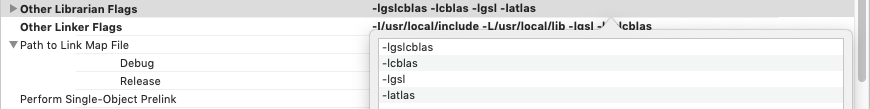
\includegraphics[width=0.9\textwidth]{figures/3.png}
  \caption{Other Librarian Flags} \label{pngsample}
\end{figure}
\begin{figure}[htbp]
  \centering
  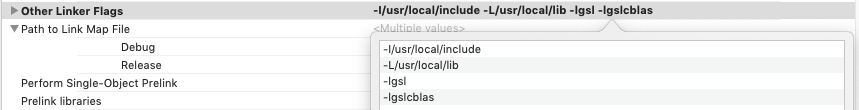
\includegraphics[width=0.9\textwidth]{figures/4.png}
  \caption{Other Linker Flags} \label{pngsample}
\end{figure}
到此,配置任务基本完成,可以使用以下样例程序测试输出Bessel函数在x=5的值。
\begin{lstlisting}
#include <stdio.h>
#include <gsl/gsl_sf_bessel.h>
int
main (void) {
double x = 5.0;
double y = gsl_sf_bessel_J0 (x); 
printf ("J0(\%g) = \%.18e\n", x, y); 
return 0;
}
\end{lstlisting}
$Out: \quad J0(5) = -1.775967713143382642e-01$\par
注意到我们的gsl安装之后是以一个文件夹的形式与其他头文件并列,所以调用时要在前面加上路径“gsl/”。
\section{错误调试}
GSL库函数在出现不同错误时会返回相应的指针,将其输出可以查看错误类型。需要调用的头文件是$gsl\_errno.h$, 程序样例如下
\begin{lstlisting}
int status = gsl_function(...)
if (status){
//如果发生了错误则运行这段程序
printf("error:%s\n",gsl_strerror(status));
}
\end{lstlisting}
\par
举例
\begin{lstlisting}
int status=gsl_sf_bessel_J0(0);
printf("error:%s\n",gsl_strerror(status));
    
Out: error:input domain error
\end{lstlisting}
在Debug不出的绝望时刻可以考虑使用。
\section{函数与常数}
本部分一般需要调用$gsl\_math.h$。\par
\subsection{常数与类型}
GSL中使用宏储存了很多常数的精确值,我们可以直接使用。
\begin{table}
\centering
\renewcommand\arraystretch{2}
\caption{常量表}
\begin{tabular}{|c|c|c|c|}
\hline
$M\_E$&$ e$&$ M\_2\_SQRTPI$&$ \frac{2}{\sqrt{\pi}}$\\\hline
$M\_LOG2E$&$ log_2{e}$&$ M\_1\_PI$&$ \frac{1}{\pi}$\\\hline
$M\_LOG10E$&$ log_{10}{e}$&$ M\_2\_PI$&$ \frac{2}{\pi}$\\\hline
$M\_SQRT2$&$ \sqrt{2}$&$ M\_LN10$&$ ln{10}$\\\hline
$M\_SQRT1\_2$&$ \sqrt{\frac{1}{2}}$&$ M\_LN2$&$ ln{2}$\\\hline
$M\_SQRT3$&$ \sqrt{3}$&$ M\_LNPI$&$ ln{e}$\\\hline
$M\_PI$&$ \pi$&$ M\_EULER$&$ Euler\;Constant\;\gamma$\\\hline
$M\_PI\_2$&$ \frac{\pi}{2}$&$ GSL\_POSINF$&$ +\frac{1.0}{0.0}$\\\hline
$M\_PI\_4$&$ \frac{\pi}{4}$&$ GSL\_NEGINF$&$ -\frac{1.0}{0.0}$\\\hline
$M\_SQRTPI$&$ \sqrt{\pi}$&$ GSL\_NAN$&$ \frac{0.0}{0.0}$\\\hline
\end{tabular}
\end{table}
举例
\begin{lstlisting}
 printf("%f",1/M_E);
 
 Out: 0.367879
\end{lstlisting}
在检查程序的时候也常常用到下面三个函数$$
int\;gsl\_isnan(const\;double \;x)
$$
$$
int\:gsl\_isinf(const\;double\; x)
$$
$$
int\;gsl\_finite(const\;double\; x)
$$
显然,他们用来检查异常值的类型,如果x是所属的类型则返回1,否则返回0。
\subsection{函数}
下面给出一些GSL常用的或者相对于一般C语言库函数特有的函数。
\begin{table}
\centering
\renewcommand\arraystretch{2}
\caption{常用函数表}
\begin{tabular}{|c|c|}
\hline

$double\;gsl\_log1p(const\;double\;x)$&返回ln(1+x)的值,对很小的x精确\\\hline
$double\;gsl\_expm1(const\;double\;x)$ &返回$e^x-1$的值,对很小的x精确\\\hline
$double\;gsl\_hypot(const\;double\;x,\;const\;double\;y)$&返回$\sqrt{x^2+y^2}$的值,且尽量避免了超限\\\hline
$double\;gsl\_hypot3(double\;x,\;double\;y,\;const\;double\;z)$&返回$\sqrt{x^2+y^2+z^2}$的值,且尽量避免了超限\\\hline
$double\;gsl\_pow\_int(double\;x,\;int\;n)$&计算$x^n$的值,且采用快速幂,效率很高\\\hline
$double\;gsl\_pow\_uint(double\;x,\;unsigned\;int\;n)$&同上,输入类型有别\\\hline
$GSL\_IS\_ODD(n)$&判断n是否为奇数,是返回1,否则为0\\\hline
$GSL\_IS\_EVEN(n)$&判断n是否为偶数,是返回1,否则为0\\\hline
$GSL\_MAX(a,b)$&返回两者的较大值\\\hline
$int\;gsl\_fcmp(double\;x,\;double\;y,\;double\;epsilon)$&判断x与y在$\epsilon$水平上是否相等,返回\\
&-1(x>y), 0(x=y), 1(x<y)\\\hline
\end{tabular}
\end{table}
GSL还包含了一些特殊函数,课程作业有可能用到,如参数为n的Bessel函数
$$
gsl\_sf\_bessel\_Jm(int\; n,\; double\; x)
$$
这些特殊函数的名称一般为$gsl\_sf\_function$,需要调用$gsl\_sf\_function.h$。




\section{变量类型的扩展}
\subsection{复数}
这部分内容一般需要调用$gsl\_complex.h$和$gsl\_complex\_math.h$。\par GSL中的复数类型为$gsl\_complex$,可以使用如下示例的两个函数定义一个复数。
\begin{lstlisting}
gsl_complex z1=gsl_complex_rect(1, 1);//直角坐标系下的横纵坐标
gsl_complex z2=gsl_complex_polar(1, M_PI/2);//极坐标下的模长和幅角
    
printf("%f+%f i\n",z1.dat[0],z1.dat[1]);//输出复数,
					//dat是复数结构中的一个元素
printf("%f+%f i\n",z2.dat[0],z2.dat[1]);

Out: 1.000000+1.000000 i
     0.000000+1.000000 i
\end{lstlisting}

而获得一个复数的性质我们有下列函数:
\begin{table}
\centering
\renewcommand\arraystretch{2}
\caption{复数返回函数表}
\begin{tabular}{|c|c|}
\hline
$GSL\_REAL(z)$&返回一个复数的实部\\\hline
$GSL\_IMAG(z)$&返回一个复数的虚部\\\hline
$gsl\_complex\_arg(z)$&返回一个复数的幅角\\\hline
$gsl\_complex\_abs(z)$&返回一个复数的模长\\\hline
$gsl\_complex\_abs2(z)$&返回一个复数模长的平方\\\hline
$gsl\_complex\_logabs(z)$&返回$ln|z|$,在$|z|\to1$的时候精确\\\hline
\end{tabular}
\end{table}

改变一个复数,我们可以使用函数
$$
void \; GSL\_SET\_COMPLEX(zp, x, y)
$$
来为z赋值,也可以使用指针单独改变实部或者虚部的值,使用
$$
GSL\_SET\_REAL(zp, x)
$$
$$
GSL\_SET\_IMAG(zp, y)
$$
也可以直接改变z的struct中二元数组dat的值。示例如下
\begin{lstlisting}
    gsl_complex z=gsl_complex_rect(1,1);
    GSL_SET_COMPLEX(&z, 2, 2);
    printf("%f+%f i\n",z.dat[0],z.dat[1]);
    z.dat[1]=0;
    printf("%f+%f i\n",z.dat[0],z.dat[1]);
    GSL_SET_IMAG(&z, -2);
    printf("%f+%f i\n",z.dat[0],z.dat[1]);
    GSL_SET_REAL(&z, -4);
    printf("%f+%f i\n",z.dat[0],z.dat[1]);

Out: 2.000000+2.000000 i
     2.000000+0.000000 i
     2.000000+-2.000000 i
     -4.000000+-2.000000 i
\end{lstlisting}

而复数的运算通过函数来完成(相对于直接编写复数类运算的表达上有些麻烦,但是图个方便吗这不是)。
\newpage

\begin{table}
\centering
\renewcommand\arraystretch{2}
\caption{复数运算函数表}
\begin{tabular}{|c|c|}
\hline
函数&返回值\\\hline
$gsl\_complex\_add(gsl\_complex\;a,\;gsl\_complex\;b)$&$a+b$\\\hline
$gsl\_complex\_sub(gsl\_complex\;a,\;gsl\_complex\;b)$&$a-b$\\\hline
$gsl\_complex\_mul(gsl\_complex\;a,\;gsl\_complex\;b)$&$ab$\\\hline
$gsl\_complex\_div(gsl\_complex\;a,\;gsl\_complex\;b)$&$\frac{a}{b}$\\\hline
$gsl\_complex\_conjugate(gsl\_complex\;z)$&$\overline{z}$\\\hline
$gsl\_complex\_inverse(gsl\_complex\;z)$&$\frac{1}{z}$\\\hline
$gsl\_complex\_negative(gsl\_complex\;z)$&$-z$\\\hline
\end{tabular}
\end{table}


常用的复变量函数列表如表5。\par

\begin{table}
\centering
\renewcommand\arraystretch{2}
\caption{复变量函数表}
\begin{tabular}{|c|c|}
\hline
函数&返回值\\\hline
$gsl\_complex\_sqrt(gsl\_complex\;z)$&$\sqrt{z}$\\\hline
$gsl\_complex\_pow\_real(gsl\_complex\;z,\;double\;x)$&$z^x$\\\hline
$gsl\_complex\_exp(gsl\_complex\;z)$&$e^z$\\\hline
$gsl\_complex\_log\_b(gsl\_complex\;z,\;gsl\_complex\;b)$&$log_bz$\\\hline
\end{tabular}
\end{table}
对于复变函数中经常使用的三角函数、反三角函数、双曲函数、反双曲函数,GSL中都有收录,调用形式诸如
$$
gsl\_complex\_cos(z)
$$
$$
gsl\_complex\_sinh(z)
$$
其中有一些对输入或输出的值有要求,比如要求为实数,跟随编译器的指引选择相应的函数名即可。

\subsection{多项式}
本部分一般需要调用$gsl\_poly.h$。\par

多项式的储存形式是数组。一个多项式和其储存在计算机中的形式是
$$
a_0+a_1x+\cdots a_nx^n
$$
$$
[a_0,a_1,a_2,\cdots,a_n]
$$
然而,对多项式本身的操作,例如求两个多项式的积,并没有在GSL中给出。本文给出可以参考的实现方式如表6。具体代码放在附录中。\par

\begin{table}[!h]
\centering
\renewcommand\arraystretch{2}
\caption{多项式操作}
\begin{tabular}{|c|c|}
\hline
函数&返回值\\\hline
double plus(double p1[], int n1, double p2[], int n2)&求n1-1次的多项式系数组p1和n2-1\\
&次的多项式系数组p2的和\\\hline
double minus(double p1[], int n1, double p2[], int n2)&求差\\\hline
double multiple(double p1[], int n1, double p2[], int n2)&求积\\\hline
double generate(double root[])&求以root中的数为根的首一多项式\\\hline
\end{tabular}
\end{table}
计算一个多项式在x点处的各种值有如下方法。
\begin{table}[!h]
\centering
\renewcommand\arraystretch{2}
\caption{多项式操作}
\begin{tabular}{|c|c|}
\hline
函数&返回值\\\hline
$gsl\_poly\_eval(double\;c[],\;int\;len,\;double\;x)$&计算实值多项式\\\hline
$gsl\_poly\_complex\_eval(double\;c[],\;int\;len,\;gsl\_complex\;z)$&计算实值复变多项式\\\hline
$gsl\_complex\_poly\_complex\_eval$&复变复值多项式\\
$(gsl\_complex\;c[],\;int\;len,\;gsl\_complex\;z)$&\\\hline
$gsl\_poly\_eval\_derivs(double\;c[],\;size\_t\;lenc,\;double\;x,$&在x处的k阶导,返回值为一个数组\\
$\;double\;res[],\;size\_t\;lenres)$&\\\hline
$gsl\_poly\_dd\_init(double\;dd[],\;double\;xa[],$&通过一个点列(横纵坐标储存在xa和ya中)\\
$double\;ya[],\;size\_t\;size)$&和均差(dd中)返回一个多项式\\\hline
\end{tabular}
\end{table}
\newpage
有关多项式方程的函数。
\begin{table}[!h]
\centering
\renewcommand\arraystretch{2}
\caption{多项式方程操作}
\begin{tabular}{|c|c|}
\hline
$int\;gsl\_poly\_solve\_quadratic(double\;a,\;double\;b,\;double\;c,\;double\;*\;x0,\;double\;*\;x1)$\\\hline
解一元二次方程\\\hline
$int\;gsl\_poly\_solve\_cubic(double\;a,\;double\;b,\;double\;c,\;double\;*\;x0,\;double\;*\;x1,\;double\;*\;x2)$\\\hline
解一元三次方程\\\hline
$int\;gsl\_poly\_complex\_solve(double\;*a,\;size\_t\;n,$\\
$gsl\_poly\_complex\_workspace\;*w,\;gsl\_complex\_packed\_ptr\;z)$\\\hline
解出多项式的所有根,返回值为一个长度为2(n-1)的数组,相邻两位依次为实部和虚部
\\\hline
\end{tabular}
\end{table}
\subsection{块}
这部分内容一般需要使用$gsl\_block.h$。\par
GSL中的向量和矩阵都是使用数据类型块(block)来表示的,其定义如下
\begin{lstlisting}
typedef struct
{
size_t size;
  double * data;
} gsl_block;
\end{lstlisting}
一个块有长度和数据,在使用时需要声明,示例如下
\begin{lstlisting}
gsl_block * b = gsl_block_alloc (100); //分配空间
printf ("length of block = %zu\n", b->size);//输出长度
printf ("block data address = %p\n", b->data);//输出数组指针
gsl_block_free (b);//释放空间
  
 Out:
 length of block = 100
 block data address = 0x804b0d8

\end{lstlisting}

\subsection{向量}
这部分内容需要使用gsl$\_$vector.h。\par
下面我们使用一个例程来说明向量使用的方法。
\newpage

\begin{lstlisting}
int i;
    gsl_vector * v = gsl_vector_alloc (3);
    for (i = 0; i < 3; i++) {
        gsl_vector_set (v, i, 1.23 + i);//分配储存空间
    }
    for (i = 0; i < 3; i++) {
        printf ("v_%d = %g\n", i, gsl_vector_get (v, i)); }//输出
    gsl_vector * u = gsl_vector_alloc (3);//再声明一个向量
    //下面很多操作要求两向量长度相同,请自行体会
    //并且,许多操作是对复数可行的,可以自行探索
    gsl_vector_set_all(u,1);//将所有位置设为1
    gsl_vector_swap(u,v);
    for (i = 0; i < 100; i++)  {//下标超限报错
        printf ("v_%d = %g\n", i, gsl_vector_get (v, i)); }//输出
    gsl_vector_swap_elements(u,1,2);//交换向量元素
    gsl_vector_reverse(u);//倒置向量
    gsl_vector_add(u,v);//相加,减乘除只需把add换成sub、mul、div
    gsl_vector_scale(u,1);//数乘
    gsl_vector_add_constant(u,1);//加常数
    gsl_vector_max(u);//找出最大值,最小值同理
    gsl_vector_min_index(u);//找出最小值的下标,最大值同理
    gsl_vector_isnull(u);//判断是否是零向量
    gsl_vector_ispos(u);//是正向量
    gsl_vector_isneg(u);//是负向量
    gsl_vector_equal(u,v);//两向量是否相等
    gsl_vector_free (v);//释放储存空间
    gsl_vector_free(u);
\end{lstlisting}
\subsection{矩阵}
这部分内容需要使用$gsl\_matrix.h$。\par
我们仍然使用一个例程来说明。

\begin{lstlisting}
int i,j;
    gsl_matrix * m = gsl_matrix_alloc (10, 3);//分配空间
    for (i = 0; i < 10; i++) for (j = 0; j < 3; j++)
        gsl_matrix_set (m, i, j, 0.23 + 100*i + j);//赋值
    for(i=0;i<10;i++){//输出
        printf("\n");
        for (j = 0; j < 3; j++)
        printf ("%g\t", i, j, gsl_matrix_get (m, i, j));}
    gsl_matrix_set_identity(m);//令m为单位对角
    gsl_matrix * ma = gsl_matrix_alloc (10, 3);//再声明一个矩阵
    gsl_matrix_set_all(ma,0);//把ma所有元素设为0
    gsl_matrix_swap(m,ma);//交换两者的值
    gsl_matrix_memcpy(m,ma);//把ma的值赋给m
    gsl_vector *v1=gsl_vector_alloc(10);
    gsl_vector *v2=gsl_vector_alloc(3);
    gsl_matrix_get_row(v2,m,2);//读取第二行的值到v2中,要求长度相同
    gsl_matrix_get_col(v1,m,2);//读取第二列
    gsl_matrix_swap_rows(m,1,2);//交换第一二行,交换列同理
    gsl_matrix_free(m);//释放空间
    gsl_matrix_add(m,ma);//对应元素相加
    gsl_matrix_mul_elements(m,ma);//对应元素相乘(不是矩阵乘法)
    gsl_matrix_max(m);//矩阵元素最大值
    int imax,jmax;
    gsl_matrix_min_index(m,&imax,&jmax);//矩阵元素最大值下标
    gsl_matrix_equal(m,ma);//判断是否相等
\end{lstlisting}


\section{线性代数}
\subsection{矩阵运算}
GSL没有定义简洁的矩阵乘法,略显美中不足,本文给出可以参考的实现\footnote{Personcom,https://blog.csdn.net/ouc$\_$09dx/article/details/19158435 },具体代码放在附录中。
\subsection{矩阵分解}
这部分内容一般需要使用$gsl\_linalg.h$。\par
GSL提供了很多矩阵分解的方式,常用的如LU分解、Cholesky分解和完全正交分解。此处以LU分解为例。
$$
int\;gsl\_linalg\_LU\_decomp(gsl\_matrix\;* A,\; gsl\_permutation\; * p,\;int \;* signum)
$$
返回时A的上三角区域(包括对角线)储存,下三角区域储存L,由于L为单位下三角,对角线可以不储存。的有时LU分解写做PA=LU,P是一个用来行置换的初等矩阵,即这里的P。signum是逆序数,可以理解为det P。如果矩阵为复数域上的,那么函数名为$gsl\_linalg\_complex\_LU\_decomp$,下面的函数同理。\par
LU分解还可以实现很多其他的功能,例如
$$
int\;gsl\_linalg\_LU\_solve(gsl\_matrix\;* LU, \;gsl\_permutation \;* p,\;gsl\_vector \;* b, gsl\_vector \;* x)
$$
可以使用LU分解来解方程组Ax=b(LUx=b)。常用的功能还有求逆矩阵、求行列式、求行列式符号(均为使用LU分解)。
$$
int\;gsl\_linalg\_LU\_invert(const\;gsl\_matrix\;*\;LU,\;const\;gsl\_permutation\;*\;p,\;gsl\_matrix\;*\;inverse)
$$
$$
double\;gsl\_linalg\_LU\_det(gsl\_matrix\;*\;LU,\;int\;signum)
$$
$$
int\;gsl\_linalg\_LU\_sgndet(gsl\_matrix\;*\;LU,\;int\;signum)
$$
\subsection{特征值}
这部分内容需要用到$gsl\_eigen.h$。\par
求不同类型的矩阵特征值只需要调用相应函数,比如对于对称矩阵有
$$
int\;gsl\_eigen\_symmv(gsl\_matrix\; * A, gsl\_vector \;* eval, gsl\_matrix \;* evec, gsl\_eigen\_symmv\_workspace\; * w)
$$
函数名只需要根据对应的矩阵类型,在编译器的引导下使用。
\section{数值积分}
这部分内容一般需要使用$gsl\_integration.h$。\par
GSL提供了一系列数值积分的函数,因为名字太长所以一般用缩写表示,缩写字母意义如下。
\begin{itemize}
\item Q - quadrature routine 
\item N - non-adaptive integrator
\item A - adaptive integrator
\item G - general integrand (user-defined) 
\item W - weight function with integrand
\item S - singularities can be more readily integrated
\item P - points of special difficulty can be supplied
\item I - infinite range of integration
\item O - oscillatory weight function, cos or sin
\item F - Fourier integral
\item C - Cauchy principal value
\end{itemize}
以一般性的自适应积分(QAG)为例

$$
int\;gsl\_integration\_qag(gsl\_function\;*\;f,\;double\;a,\;double\;b,\;double\;epsabs,\;double\;epsrel,
$$
$$
size\_t\;limit,\;int\;key,\;gsl\_integration\_workspace\;*\;workspace,\;double\;*\;result,
double\;*\;abserr)
$$
参数意义分别是:函数,积分上下限,绝对和相对误差,积分区间个数上限,积分方式选择(使用哪一种高斯积分,key的值可以选择整数1-6,在数值计算课程应用范围内区别不大),积分储存空间声明,积分结果,积分结果绝对误差。给出例程如下。\par
\begin{lstlisting}
gsl_integration_workspace * w//声明空间
= gsl_integration_workspace_alloc (1000);
  double result, error;
  double expected = -4.0;
  double alpha = 1.0;
  gsl_function F;
  F.function = &f;
  F.params = &alpha;
  gsl_integration_qags 
  (&F, 0, 1, 0, 1e-7, 1000/*声明了1000,所以最多设为1000*/,
   w, &result, &error);
printf ("result = % .18f\n", result);
printf ("exact result = % .18f\n", expected);
\end{lstlisting}
使用GSL提供的数值积分,既可以对自己的程序起到验证性作用,又可以通过比较不同类型积分得到的绝对误差来比对不同方法的特性,不失为一种好的拓展学习的方式。
\section{插值}
这部分内容一般需要使用$gsl\_interp.h$和$gsl\_spline.h$。\par
对于一位差值,GSL提供很多函数如线性、样条和牛顿,牛顿我们在之前的多项式部分已经提到。我们仍旧用一个例程来说明。
\begin{lstlisting}
int i;
double xi, yi, x[10], y[10];//给出差值点列
for (i = 0; i < 10; i++) {
x[i] = i + 0.5 * sin (i);
y[i] = i + cos (i * i);
}
  {
    gsl_interp_accel *acc
      = gsl_interp_accel_alloc ();//声明差值和加速所需要的储存空间
    gsl_spline *spline
      = gsl_spline_alloc (gsl_interp_cspline, 10);
    gsl_spline_init (spline, x, y, 10);//初始化
for (xi = x[0]; xi < x[9]; xi += 0.01) {
        yi = gsl_spline_eval (spline, xi, acc);//计算差值
printf ("%g %g\n", xi, yi); }
    gsl_spline_free (spline);//释放空间
    gsl_interp_accel_free (acc);
  }
\end{lstlisting}
不过事实上差值的部分使用C的意义并不大,因为函数只会返回差值点处的值。而且如果想要做出差值图像,需要找到a.out,又需要学习更多知识,所以此处略微提及。
\begin{appendix}
\section{多项式操作}
\begin{lstlisting}
double *plus(double p1[],int l1,double p2[],int l2){//加函数
    int l=gsl_max(l1, l2);
    if(l>l1){
        double *temp;
        int tem;
        temp=p2;
        p2=p1;
        p1=temp;
        tem=l2;
        l2=l1;
        l1=tem;
    }
    double result[l];
    for(int i=0;i<l;i++){result[i]=p1[i];}
    for(int i=0;i<l2;i++){result[i]+=p2[i];}
    while(result[l-1]==0&&l>0){l=l-1;}
    double *p;
    p=(double*)malloc(sizeof(double)*l);
    return p;
}
\end{lstlisting}
\begin{lstlisting}
double *minus(double p1[],int l1,double p2[],int l2){//减函数
    int l=gsl_max(l1, l2);
    int sig=1;
    if(l>l1){
        double *temp;
        int tem;
        temp=p2;
        p2=p1;
        p1=temp;
        tem=l2;
        l2=l1;
        l1=tem;
        sig=-1;
    }
    double result[l];
    for(int i=0;i<l;i++){result[i]=p1[i];}
    for(int i=0;i<l2;i++){result[i]+=p2[i];
    result[i]=result[i]*sig;}
    while(result[l-1]==0&&l>0){l=l-1;}
    double *p;
    p=(double*)malloc(sizeof(double)*l);
    return p;
}
\end{lstlisting}
\begin{lstlisting}
double *multiple(double p1[],int l1,double p2[],int l2){//乘函数
    int l=l2+l2-1;
    double *p;
    p=(double*)malloc(sizeof(double)*l);
    for(int i=0;i<l;i++){p[i]=0;}
    for(int i=0;i<l;i++){
        for(int j=0;j<l1;j++){
            for(int k=0;k<l2;k++){
                if(j+k==i){
                    p[i]+=p1[j]*p2[k];
                }
            }
        }
    }
    return p;
}
\end{lstlisting}
\begin{lstlisting}
double *generate(double root[],double n){//通过根生成多项式
    double *c;
    c=(double*)malloc(sizeof(double)*(n+1));
        c[0]=-root[0];c[1]=1;
    for(int i=2;i<n+1;i++){
        double temp[2];
        temp[1]=1;temp[0]=-root[i-1];
        c=multiple(c,i,temp,2);
    }
    return c;
}
\end{lstlisting}
为了防止丢失空间,以上四个函数务必在使用之后将使用malloc的空间释放,示例如下。
\begin{lstlisting}
double *c;
    c=generate(a,2);
    //检查malloc是否成功,可以不写
    if(c==NULL){
        perror("error");
        exit(1);
    }
    释放空间
    free(c);
\end{lstlisting}
\section{矩阵乘法}
\begin{lstlisting}
gsl_matrix *gsl_matrix_mul(gsl_matrix *a,gsl_matrix *b){//矩阵乘法
	gsl_matrix *c=gsl_matrix_alloc(a->size1,b->size2);
	for (size_t i=0;i<a->size1;i++){
	for (size_t j=0;j<b->size2;j++){
		double sum=0.0;
		for (size_t k=0;k<b->size1;k++){
		sum+=gsl_matrix_get(a,i,k)*gsl_matrix_get(b,k,j);}
		gsl_matrix_set(c,i,j,sum);
		}
		return c;
	}
\end{lstlisting}
\end{appendix}

\end{document}
